\documentclass[10pt, a4paper]{article}

\usepackage[margin=2cm]{geometry}
\usepackage{amsmath}
\usepackage{amssymb}
\usepackage{graphicx}
\usepackage{booktabs}
\usepackage{multirow}
\usepackage{subcaption}

\title{\textbf{HW6 - Explainable AI}}
\author{Vanja Stojanovi\'c}
\date{May 2026}

\begin{document}
\maketitle

\section{LIME on \texttt{toydataset.csv}}

The dataset has 5000 observations with two continuous features $x_1, x_2 \in [-1, 0.5]$, one categorical feature $x_3 \in \{1, 2, 3\}$ (counts $1653 / 1739 / 1608$), and a continuous target $y \in [0.10, 3.33]$ with $\bar y = 1.52$. The marginal $\bar y \mid x_3$ already separates the categories ($1.84 / 1.36 / 1.35$ for $x_3 = 1 / 2 / 3$), and the colour bands in Fig.~\ref{fig:overview} show that $y$ depends non-monotonically on $x_1$ (high $y$ near both $x_1 \approx 0.5$ and $x_1 \approx -1$) and is only weakly dependent on $x_2$.

The black-box is a Random Forest regressor (500 trees, \texttt{min\_samples\_leaf}=5, seed 42) fit on the raw $(x_1, x_2, x_3)$ matrix. RF needs no scaling and handles ordinal-encoded $x_3$ by splitting on it directly, so the same representation is used by both the model and the LIME sampler. With an 80/20 train/test split, 5-fold CV on the train side gives $R^2 = 0.866 \pm 0.013$ (MSE $0.046 \pm 0.003$), and the held-out set gives $R^2 = 0.878$ (MSE $0.042$). The model is the target of explanation; no claim is made that it recovers the data-generating process.

For each query point $x$, LIME draws $N = 5000$ perturbed points. Continuous features are sampled independently from $\mathcal N(\mu_j, \sigma_j^2)$ using training statistics, and $x_3$ is sampled from its empirical frequencies. This is the global sampling scheme of the reference LIME library; an alternative is $\mathcal N(x_j, \sigma_{\text{loc}}^2)$ centred on the instance, which gives higher fidelity but more variance across seeds. The interpretable representation is $z \in \{0,1\}^3$: continuous features are discretized into training-set quartiles with $z_j = 1$ iff the perturbed value falls in the same bin as $x$, and for $x_3$, $z_j = 1$ iff the perturbed category equals $x_3$. Coefficients then read directly as "being in the instance's bin for feature $j$ contributes this many $y$-units". Four bins balance resolution against samples per cell; finer binning would shrink each cell's effective sample size.

Sample weights are $\pi_x(x') = \exp(-d^2 / \sigma_K^2)$ with $d$ Euclidean in standardized space (continuous features in $z$-score units, categorical mismatch contributing one unit of distance) and $\sigma_K = 0.75 \sqrt{d_{\text{feat}}}$, the LIME default, which sets the effective neighbourhood radius. The surrogate is a weighted Lasso with $\alpha = 0.01$, small enough to retain non-trivial effects but large enough to zero out features with no local signal. Repeating the explanations under 5 different seeds gives coefficient std $\le 0.025$ on every instance, so what follows is well-determined.

\begin{figure}[h]
\centering
\begin{subfigure}{0.95\textwidth}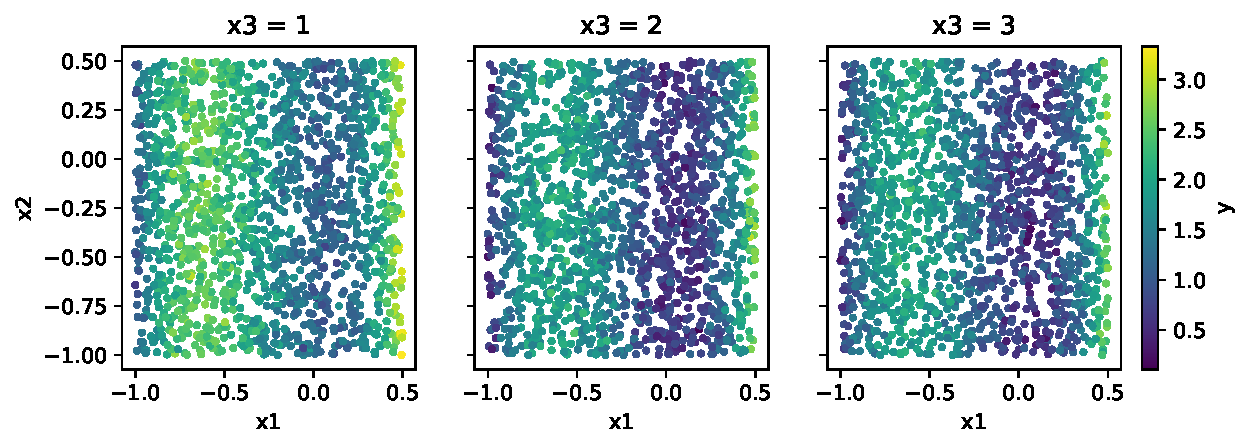
\includegraphics[width=\linewidth]{build/data_overview.pdf}\end{subfigure}\\[0.3em]
\begin{subfigure}{0.95\textwidth}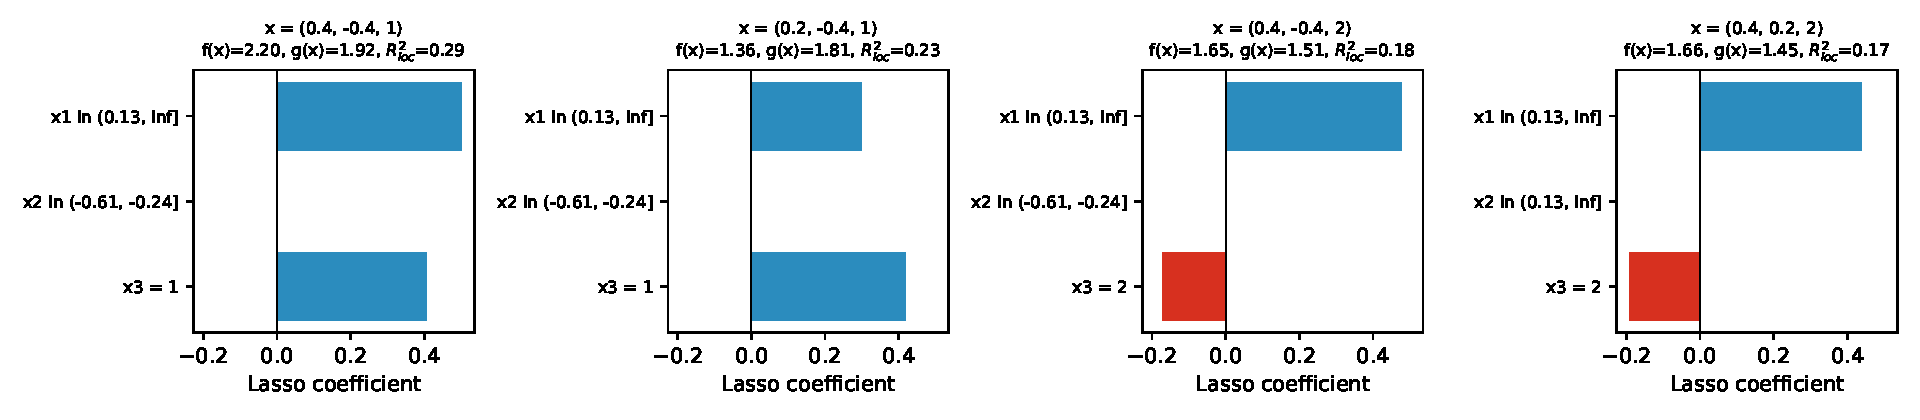
\includegraphics[width=\linewidth]{build/lime_explanations.pdf}\end{subfigure}
\caption{Top: $y$ vs.\ $(x_1, x_2)$ split by $x_3$, full data set. Bottom: LIME bar plots, blue $= +$, red $= -$. Each panel shows the black-box prediction $f(x)$, the surrogate prediction $g(x)$, and the kernel-weighted local $R^2$ of the surrogate.}
\label{fig:overview}
\end{figure}

\begin{table}[h]
\centering
\small
\caption{LIME explanations of the four query points. Coefficients $\beta_j$ are those of the weighted Lasso on the binary $z$. The instance has $z = (1, 1, 1)$ by construction, so $g(x) = \beta_0 + \sum_j \beta_j$.}
\label{tab:lime}
\begin{tabular}{cccccccc}
\toprule
$x_1$ & $x_2$ & $x_3$ & $f(x)$ & $\beta_0$ & $\beta_{x_1 \text{ bin}}$ & $\beta_{x_2 \text{ bin}}$ & $\beta_{x_3 = \text{cat}}$ \\
\midrule
$0.4$ & $-0.4$ & $1$ & $2.20$ & $1.02$ & $+0.50$ (top) & $0.00$ (Q2)  & $+0.41$ ($x_3{=}1$) \\
$0.2$ & $-0.4$ & $1$ & $1.36$ & $1.09$ & $+0.30$ (top) & $0.00$ (Q2)  & $+0.42$ ($x_3{=}1$) \\
$0.4$ & $-0.4$ & $2$ & $1.65$ & $1.21$ & $+0.48$ (top) & $0.00$ (Q2)  & $-0.17$ ($x_3{=}2$) \\
$0.4$ & $\phantom{-}0.2$ & $2$ & $1.66$ & $1.21$ & $+0.44$ (top) & $0.00$ (top) & $-0.19$ ($x_3{=}2$) \\
\bottomrule
\end{tabular}
\end{table}

All four instances have $x_1 > 0.13$, the top quartile, and LIME assigns this bin a positive coefficient ($+0.30$ to $+0.50$), matching the high-$y$ band at $x_1 \approx 0.5$ visible in Fig.~\ref{fig:overview}. The $x_2$ coefficient is shrunk to zero by Lasso on every instance: there is no local $x_2$ gradient at these query points, consistent with the weak visual $x_2$ dependence. The $x_3$ coefficient is $+0.4$ when the instance has $x_3 = 1$ and $-0.18$ when $x_3 = 2$, matching the marginal $\bar y \mid x_3$ gap.

One limitation of quartile-LIME is visible in the table. The first two instances share an identical $z = (1, 1, 1)$ because both have $x_1$ in the top quartile, $x_2$ in Q2, and $x_3 = 1$, so the surrogate assigns them the same explanation, yet $f(x)$ differs by $0.84$. This is the source of the low local $R^2$ (0.17 to 0.29 across instances): the binary surrogate cannot resolve the $x_1 = 0.4 \to 0.2$ gradient inside the top quartile, where the data-overview plot shows a steep drop. Refusing discretization, and using $z$-scored $x'$ directly as surrogate features instead, trades this readability for fidelity.

\clearpage

\section{Shapley values}

The Shapley value of feature $j$ at point $x$ is
$$
\varphi_j(x) \;=\; \sum_{S \subseteq N \setminus \{j\}}
   \frac{|S|!\,(d - |S| - 1)!}{d!}\, \bigl(v(S \cup \{j\}) - v(S)\bigr),
\qquad
v(S) \;=\; \mathbb E_{X \sim p}\!\bigl[f(X_S = x_S, X_{N \setminus S})\bigr],
$$
the average marginal contribution of $j$ over a uniformly random ordering of the features. Under the assumption that features are independent the coalition value $v(S)$ is the interventional expectation above, estimated by Monte Carlo over a background sample $B \subset X_{\text{train}}$: hold features in $S$ fixed at $x_S$, replace the others with the rows of $B$, average the black-box prediction. We use $|B| = 500$ rows drawn uniformly from the training split; the variance of $\hat v(S)$ is already an order of magnitude below the inter-feature differences at this size.

With $d = 3$ the $2^d = 8$ coalition values can be enumerated exactly, so the only Monte-Carlo step is the background average. Two equivalent paths recover the same numbers and we implement both: the exact subset-weighted sum above, and a permutation-Monte-Carlo (Strumbelj and Kononenko, 2014) that draws random feature orderings and chains $b \to (b \text{ with } x \text{ inserted along } \pi) \to \cdots \to x$, accumulating one-step prediction differences. With $5000$ permutations the latter matches the exact value to within $0.006$ on every feature for every query point, which is a useful sanity check on the implementation.

\begin{figure}[h]
\centering
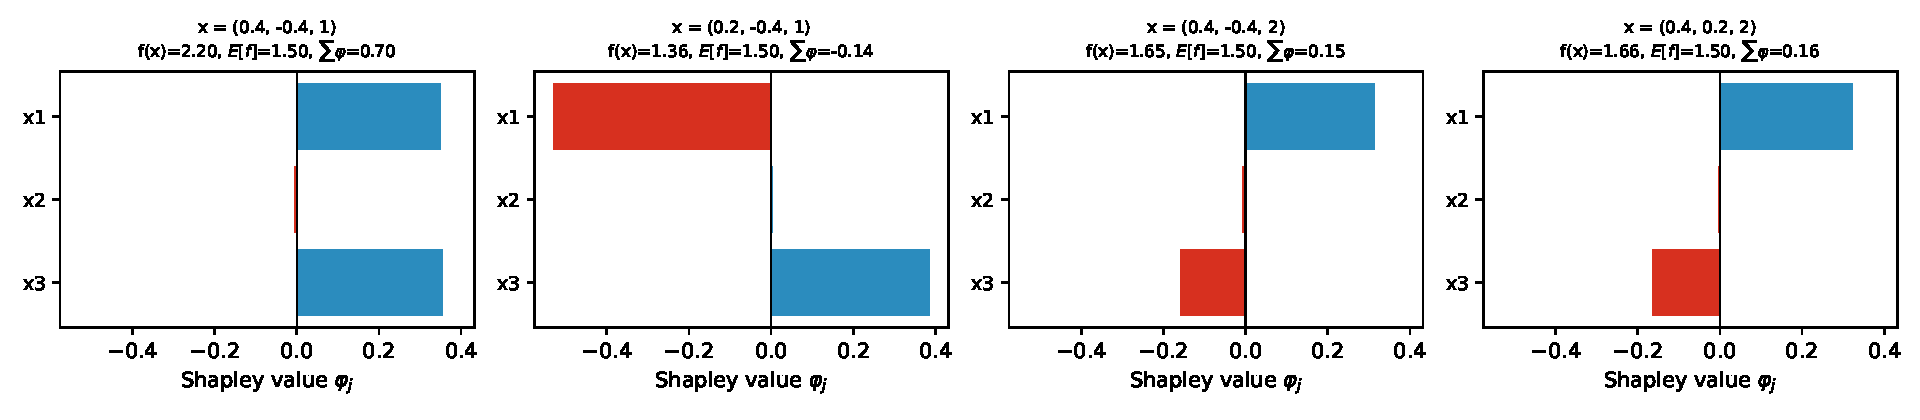
\includegraphics[width=0.96\textwidth]{build/shapley_explanations.pdf}
\caption{Shapley values $\varphi_j(x)$ for the four query points. Each title shows $f(x)$, the baseline $\mathbb E[f] = 1.50$, and $\sum_j \varphi_j$. By the efficiency axiom $f(x) - \mathbb E[f] = \sum_j \varphi_j$ exactly, and indeed every panel satisfies this to numerical precision.}
\label{fig:shap}
\end{figure}

\begin{table}[h]
\centering
\small
\caption{Exact Shapley values under feature independence, $\mathbb E[f] = 1.499$. The right-most column verifies the efficiency axiom $\sum_j \varphi_j = f(x) - \mathbb E[f]$ (to numerical precision).}
\label{tab:shap}
\begin{tabular}{ccccccccc}
\toprule
$x_1$ & $x_2$ & $x_3$ & $f(x)$ & $\varphi_{x_1}$ & $\varphi_{x_2}$ & $\varphi_{x_3}$ & $\sum_j \varphi_j$ & $f - \mathbb E[f]$ \\
\midrule
$0.4$ & $-0.4$ & $1$ & $2.199$ & $+0.349$ & $-0.004$ & $+0.355$ & $+0.700$ & $+0.700$ \\
$0.2$ & $-0.4$ & $1$ & $1.360$ & $-0.530$ & $+0.004$ & $+0.387$ & $-0.139$ & $-0.139$ \\
$0.4$ & $-0.4$ & $2$ & $1.646$ & $+0.313$ & $-0.007$ & $-0.159$ & $+0.147$ & $+0.147$ \\
$0.4$ & $\phantom{-}0.2$ & $2$ & $1.656$ & $+0.323$ & $-0.003$ & $-0.163$ & $+0.157$ & $+0.157$ \\
\bottomrule
\end{tabular}
\end{table}

Shapley resolves what LIME with quartile bins cannot. The two instances $(0.4, -0.4, 1)$ and $(0.2, -0.4, 1)$ produce identical $z$ vectors and so identical LIME explanations, but their Shapley attributions for $x_1$ differ in sign and magnitude ($+0.35$ vs.\ $-0.53$). The latter is consistent with the colour map in Fig.~\ref{fig:overview}: at $x_1 = 0.2$ the model sits in the low-$y$ trough between the two yellow bands, so $x_1$ contributes negatively relative to baseline; at $x_1 = 0.4$ the model is close enough to the right-hand yellow band that $x_1$ contributes positively. The $x_3$ attributions are $+0.36 / +0.39 / -0.16 / -0.16$, the same sign pattern as the marginal $\bar y \mid x_3$ gap and within $0.05$ of the LIME categorical effects. The $x_2$ attributions are below $0.01$ in absolute value on all four instances, agreeing with the LIME finding that $x_2$ carries no signal locally.

The two methods answer different questions, which explains both their agreement on the $x_3$ effect and their divergence on samples 1 vs.\ 2. LIME fits a sparse linear surrogate to a kernel-weighted neighbourhood, so its coefficients describe a local linear trend in $z$ space; Shapley distributes the gap $f(x) - \mathbb E[f]$ across features by averaging marginal contributions over all coalition orderings, with no surrogate model and no discretization step. On this dataset Shapley is closer to what one wants from a feature attribution: it is signed and continuous in $x$, it satisfies efficiency by construction, and it does not collapse two different $x_1$ values to the same bin.

\end{document}
